\documentclass[xcolor=pdftex,dvipsnames,table,final]{beamer}
\mode<presentation>
{
  \usetheme{PosterCERG}
}
% size in width and height is in cm
% Arch D: 24"x36" use 60.96 x 91.44 Typical size for our printer, use 3 columns, scale=0.8 to fit more text
% each column should be 0.3\linewidth
% Arch E: 36"x48" use 91.44 x 121.92 OK for FedexKinko, use 4 columns
% each column should be 0.22\linewidth
\usepackage[orientation=portrait,size=custom,width=76.2,height=106.68,scale=1]{beamerposter}
% DATE-2016 Poster format
% DIN-A0-Portrait ----1189mm X 841mm or 118.9cm x 84.1cm or 46.8in x 33.1in 
%\usepackage[orientation=portrait, size=custom, width=84.1, height=118.9 scale=1.0]{beamerposter}sd
\usepackage{multirow,wrapfig}
\usepackage[labelformat=empty,justification=centering]{caption}
\usepackage{tikz}
\usepackage{lmodern}
\usepackage{multirow}
\usepackage{listings}
\usetikzlibrary{fit,arrows,calc,positioning}
%\usepackage{wrapfig}
%%%%%%%%%%% Additional packages-Panci
\usepackage[T1]{fontenc}

\definecolor{ocean}{RGB}{0,205,255}
\definecolor{beamerbackground}{rgb}{0.5,0.5,0.3}
\newcommand{\rb}[1]{\raisebox{1.3ex}[-1.3ex]{#1}}

\newcommand{\urlwofont}[1] { \urlstyle{same}\url{#1} }
     
\graphicspath{{figures/}}
\title{\LARGE eXtended eXternal Benchmarking eXtension\\ \vspace{0.5ex}(XXBX)}
\author{Matthew R. Carter \and Raghurama R. Velegala \and John Pham \and Jens-Peter Kaps}%\vspace{-2ex}
\institute{\vspace{-1ex}Department of Electrical and Computer Engineering, George Mason University, Fairfax, Virginia 22030, USA }
\date{March}

\begin{document}
\lstset{%
  basicstyle=\ttfamily,
  language=bash,
  commentstyle=\color{tabutter},
  keywordstyle=\color{black},
  numberstyle=\color{cergbg1},
  stringstyle=\color{ta3orange},
  identifierstyle=\color{cergbg1}
}
\begin{frame}[fragile]{} 
  \begin{columns}[t]
% ---------------------------------------------------------------------------
%   FIRST COLUMN
% ---------------------------------------------------------------------------
    \begin{column}{.31\linewidth}

% ---------------------------------------------------------------------------
      \begin{block}{Abstract}
      Text
      \end{block}

% ---------------------------------------------------------------------------
      \begin{block}{Motivation}
      IOT
      \end{block}
	 
%---------------------------------------------------------------------------------
      \begin{block}{Benchmarking Tools}
        \begin{itemize}
          \item SUPERCOP
          \item XBX
        \end{itemize}

        \begin{center}
        \begin{minipage}[t]{0.9\linewidth}  
        \setbeamercolor{padding}{fg=white, bg=cergbg1}
        \begin{beamercolorbox}[rounded=true]{padding}
          \textbf{Missing Features}
          \begin{itemize}
            \item ROM Usage
            \item RAM Usage
            \item Power Consumption
          \end{itemize}
        \end{beamercolorbox}
        \end{minipage}
        \end{center}
      \end{block}
%-----------------------------------------------------------------------------------
      \begin{block}{Metrics}
        {\large\textbf{Throughput}}
        \begin{itemize}
          \item Item 
        \end{itemize}
        {\large\textbf{RAM Usage}}
        \begin{itemize}
          \item Item 
        \end{itemize}
        {\large\textbf{ROM Usage}}
        \begin{itemize}
          \item Item 
        \end{itemize}
        {\large\textbf{Power Consumption}}
        \begin{itemize}
          \item Item 
        \end{itemize}
      \end{block}
        
%---------------------------------------------------------------------------------
    \end{column}
% ---------------------------------------------------------------------------
%   SECOND COLUMN
% ---------------------------------------------------------------------------
    \begin{column}{.31\linewidth}
   
% ---------------------------------------------------------------------------
      
% ---------------------------------------------------------------------------
      \begin{block}{XXBX}
        {x\color{red}X}tended e{\color{red}X}ternal {\color{red}B}enchmarking 
        e{\color{red}X}tention, is extends the XBX by 
        \begin{itemize}
          \item List of differences to XBX
        \end{itemize}
        \begin{center}
          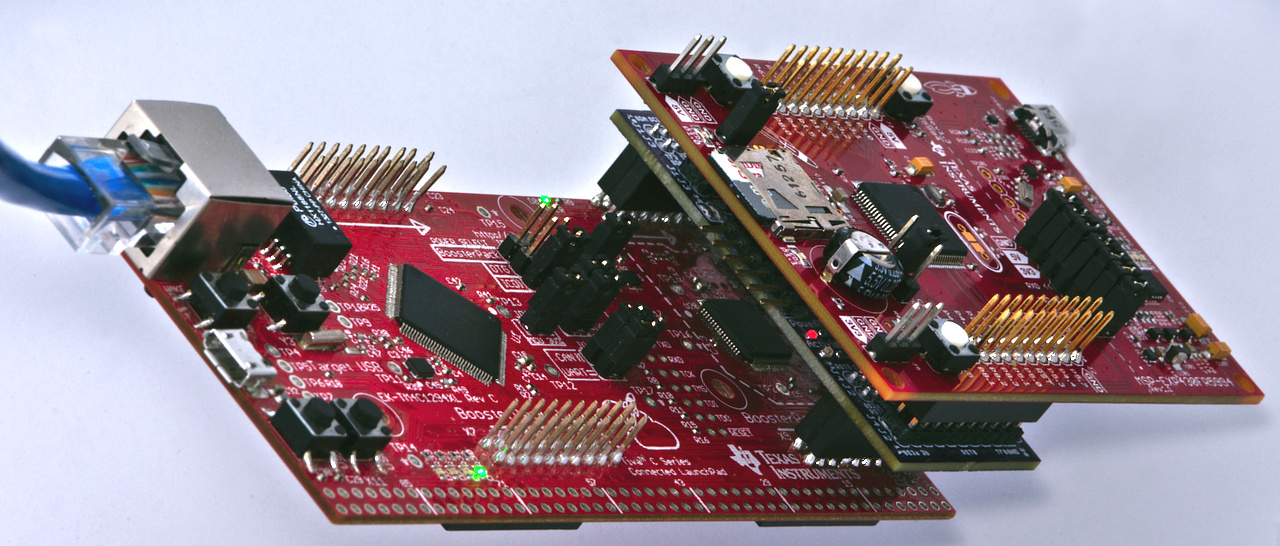
\includegraphics[scale=1.5]{../figures/xxbx-tilted}
        \end{center} 
      \end{block}
% ---------------------------------------------------------------------------
      \begin{block}{Main Components of XXBX}
        \begin{center}
          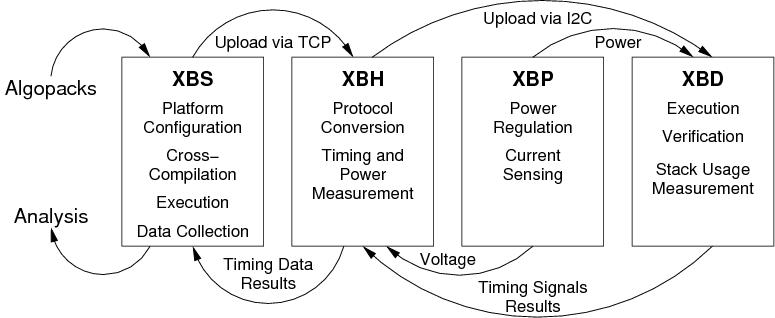
\includegraphics[scale=1.5]{../figures/xxbx_block}
        \end{center} 
        \begin{itemize}
          \item XXBX Software -- XBS 
          \begin{itemize}
            \item item 
          \end{itemize}
          \item XXBX Harness -- XBH 
          \begin{itemize}
            \item item 
          \end{itemize}
          \item XXBX Power Shim -- XBP
          \begin{itemize}
            \item item 
          \end{itemize}
          \item XXBX Device Under Test -- XBD
          \begin{itemize}
            \item item 
          \end{itemize}
        \end{itemize}
      \end{block}
     
% ---------------------------------------------------------------------------
      \begin{block}{Supported XBDs}
    \begin{tabular}{l|l|ll|rrc|rr|r}
    Board            & Manuf.    & CPU            &  ISA        & Bus    &$f$       &HW   & ROM & RAM \\ \hline
%    Homemade         & Atmel     & ATmega1284P    &  AVR        &  8-bit &  20\,MHz &     &     &        \\
    MSP-EXP430F5529  & TI        & MSP430F        &  MSP430X    & 16-bit &  25\,MHz &     &   12kB &  10kB  \\
    MSP-EXP430FR5994 & TI        & MSP430FR       &  MSP430X    & 16-bit &  16\,MHz & AES &  256kB &   8kB  \\
    MSP-EXP432P401R  & TI        & ARM Cortex M4F &  ARMv7E-M   & 32-bit &  48\,MHz & AES &  256kB &  64kB  \\
    EK-TM4C123GXL    & TI        & ARM Cortex M4F &  ARMv7E-M   & 32-bit &  80\,MHz &     &  256kB &  32kB  \\ 
    EK-TM4C129EXL    & TI        & ARM Cortex M4F &  ARMv7E-M   & 32-bit & 120\,MHz & AES & 1024kB & 256kB  \\ 
    NUCLEO-F091RC    & STM       & ARM Cortex M0  &  ARMv6-M    & 32-bit &  48\,MHz &     &  256kB &  32kB  \\
    NUCLEO-F103RB    & STM       & ARM Cortex M3  &  ARMv7-M    & 32-bit &  72\,MHz &     &  128kB &  20kB  \\
%    chipKIT uC32     & Microchip & PIC32MX3xx     &  MIPS32 M4K & 32-bit &  80\,MHz &     &     &     &   \\
    \end{tabular}


        \begin{center}
          \includegraphics[scale=1.5]{../figures/fobos-dac}
        \end{center} 

          \begin{itemize}
            \item FOBOS Acquisition Hardware contains 
            \begin{itemize}
              \item VHDL for the \textbf{Control Board} to interface with DUT,
              \item VHDL-wrapper for the \textbf{DUT board} to instantiate a user provided algorithm, and
              \item Connector description.
            \end{itemize}
            \item FOBOS Acquisition Software is written in Python and 
            \begin{itemize}
              \item Controls FOBOS Acquisition Hardware,
              \item Controls measurement equipment, and
              \item Stores measurements and setup information.
            \end{itemize}
          \end{itemize}
       \end{block}
     
% ---------------------------------------------------------------------------
      \begin{block}{FOBOS Hardware}
        \vspace{-1ex}
        \begin{center}
          \includegraphics[width=0.9\linewidth]{../figures/FOBOS-label}
        \end{center} 
        \begin{itemize}
          \item FOBOS Control can be Digilent Nexys2 or Nexys3, soon Nexys4.
        \end{itemize}
        \vspace{-0.2ex}
       \end{block}
     
% ---------------------------------------------------------------------------
      \begin{block}{Acquisition Control}
        \begin{center}
          \includegraphics[scale=1.5]{../figures/data_acq}
        \end{center} 
        \begin{itemize}
          \item Control Board sends Key and Plaintext to the DUT.
          \item After DUT receives all data, the Control Board generates the trigger.
          \item The trigger indicates that the cryptographic algorithm has started
                and initiates capture of data by the oscilloscope.
        \end{itemize}
       \end{block}
     
% ---------------------------------------------------------------------------
          
% ---------------------------------------------------------------------------
    \end{column}
% ---------------------------------------------------------------------------
%   THIRD COLUMN
% ---------------------------------------------------------------------------
   \begin{column}{.31\linewidth}
    
% ---------------------------------------------------------------------------
       \begin{block}{Power Measurement}
        \begin{minipage}{0.69\linewidth}
		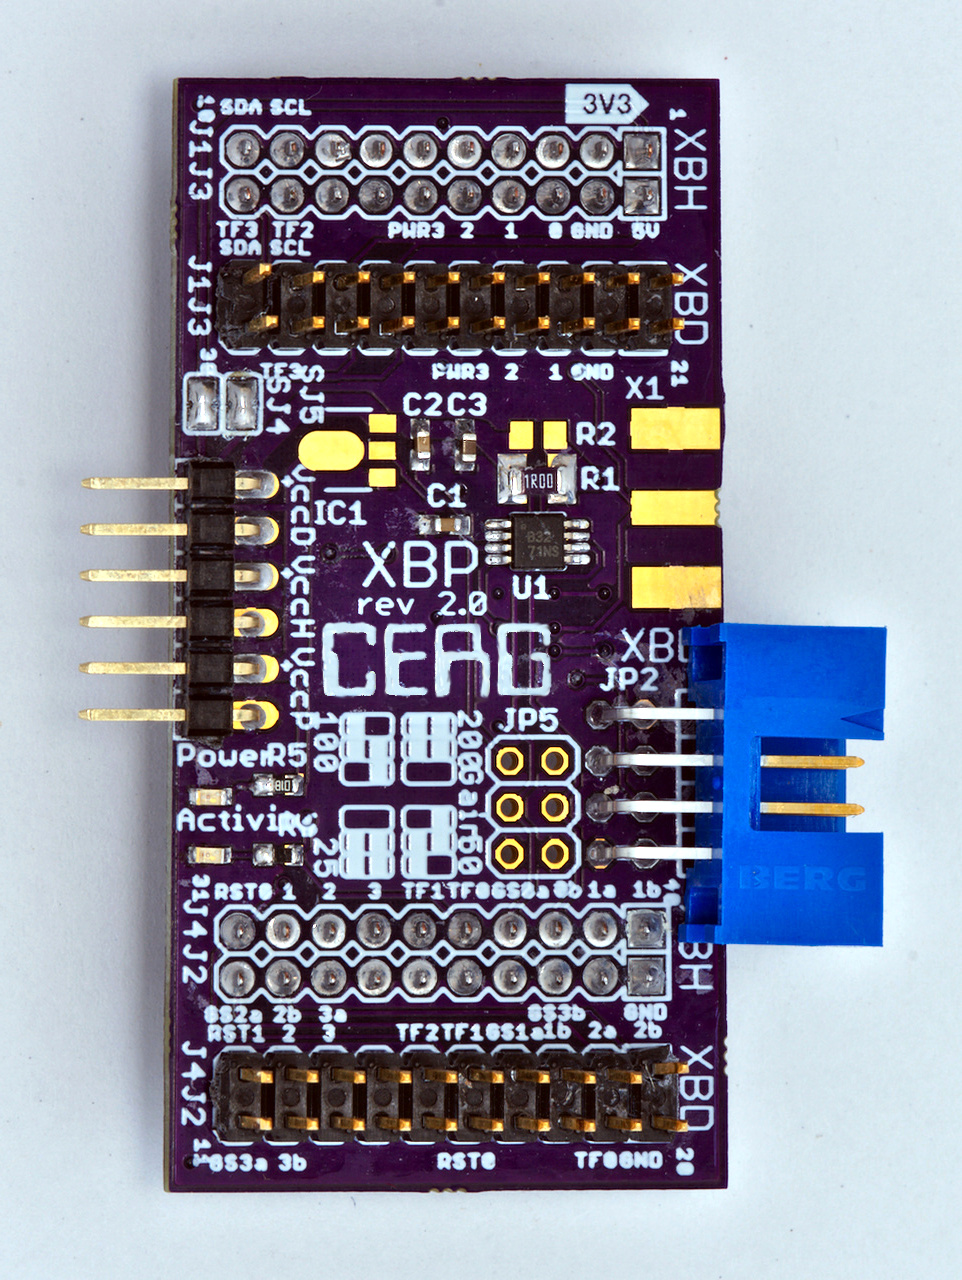
\includegraphics[scale=1.5]{../figures/xbp-full-top90}
        \end{minipage}
	\hspace{-5ex}
	\begin{minipage}{0.31\linewidth}
          \begin{itemize}
            \item Fits between XBH and XBD
            \item Contains I$^2$C pull-ups
            \item Space for power regulator
            \item Supports XBDs with 1.2\,V--5\,V
            \item Eagle files in git
          \end{itemize}
	\end{minipage} 
        \begin{center}
          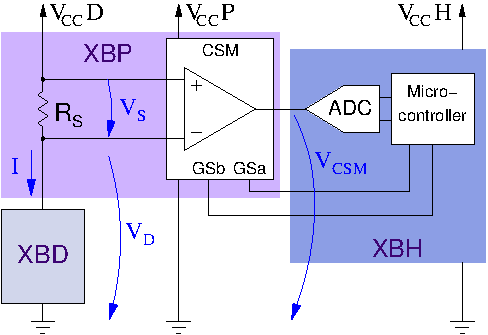
\includegraphics[scale=1.5]{../figures/ina225}
        \end{center} 
       \end{block}
% ---------------------------------------------------------------------------
       \begin{block}{Analysis Workflow}
        \vspace{-1ex}
        \begin{center}
          \includegraphics[scale=1.5]{../figures/data_anl}
        \end{center} 
        \vspace{-1ex}
        \begin{enumerate}
          \item Statistics Module
          \begin{itemize}
            \item Statistics can identify outliers in traces and samples across traces.
          \end{itemize}
          \item Post-Processing Module
          \begin{itemize}
            \item The main goal of these modules is to reduce the amount of data that 
                  has to be analyzed by the SCA Module.
          \end{itemize}
          \item SCA Module
          \begin{itemize}
            \item User can test his/her own power model using a library of state-of-the art side channel
                  distinguishers.
            \item FOBOS supports CPA using Spearman, Pearson, ANOVA \& MIA.
          \end{itemize}
        \end{enumerate}

       \end{block}
% ---------------------------------------------------------------------------
       \begin{block}{Signal Alignment}
        \begin{minipage}[t]{0.49\linewidth}
          \includegraphics[scale=2.4]{../figures/tracealingment}
        \end{minipage}%
        \begin{minipage}[t]{0.49\linewidth}
         \vspace{-4cm}
         \begin{itemize}
          \item The recorded trigger signal is used by FOBOS Analysis to align the
                power traces.
         \end{itemize} 
        \end{minipage}
       \end{block}
% ---------------------------------------------------------------------------
       \begin{block}{Sample Space Disposition}
        \begin{minipage}[t]{0.49\linewidth}%
		\includegraphics[width=0.9\linewidth]{../figures/oscilloscope-sample-window}
        \end{minipage}%
        \begin{minipage}[t]{0.49\linewidth}%
          \vspace{-6.5cm}% 
          \begin{itemize}
            \item User can select any part of the trace for further analysis.
            \item Reduces computation time.
          \end{itemize} 
          \begin{center}
            \setbeamercolor{padding}{fg=white, bg=cergbg3}
            \begin{beamercolorbox}[rounded=true]{padding}%
               \footnotesize%
              \begin{lstlisting}
WINDOW_START_POINT = 100
SAMPLE_WINDOW = 1000
              \end{lstlisting}
            \end{beamercolorbox}
          \end{center}
        \end{minipage}
       \end{block}
% ---------------------------------------------------------------------------
       \begin{block}{CAESAR Results}
        \begin{center}
        { \small%
          \renewcommand\tabcolsep{4pt}% 
          \rowcolors{3}{RoyalBlue!5}{RoyalBlue!20}%
          \begin{tabular}{|r||c|c|c|c||c|c}\hline
            \rowcolor{RoyalBlue!20}%
              & \multicolumn{4}{>{\columncolor{RoyalBlue!20}}c||}{\textbf{SASEBO}} 
              & \multicolumn{2}{>{\columncolor{RoyalBlue!20}}c}{\textbf{SAKURA}}      \\ 
            \rowcolor{RoyalBlue!20}%
            \rb{\textbf{Board}}   &          & \textbf{G} & \textbf{GII}  & \textbf{B}   & \textbf{X}   & \textbf{G}    \\ \hline
            \textbf{Control}      & Virtex-2 & Virtex-2   &               &              &              &               \\
            \rowcolor{RoyalBlue!5}%
            \textbf{FPGA}         & Pro      & Pro        &\rb{Spartan-3A}&\rb{Stratix-2}&\rb{Spartan-6}&\rb{Spartan-6} \\
            \rowcolor{RoyalBlue!20}%
            \textbf{DUT}          & Virtex-2 & Virtex-2   &               &              &              &               \\
            \textbf{FPGA}         & Pro      & Pro        &\rb{Virtex-5}  &\rb{Stratix-2}&\rb{Kintex-7} &\rb{Spartan-6} \\ 
            \textbf{Techn.}       
              & \multicolumn{1}{>{\columncolor{RoyalBlue!5}}r|}{130\,nm}  
              & \multicolumn{1}{>{\columncolor{RoyalBlue!5}}r|}{130\,nm}  
              & \multicolumn{1}{>{\columncolor{RoyalBlue!5}}r|}{65\,nm}        
              & \multicolumn{1}{>{\columncolor{RoyalBlue!5}}r||}{90\,nm}       
              & \multicolumn{1}{>{\columncolor{RoyalBlue!5}}r|}{28\,nm}    
              & \multicolumn{1}{>{\columncolor{RoyalBlue!5}}r}{45\,nm} \\       
                                  &          & RS232,     &               & RS232,       &              &               \\
            \rowcolor{RoyalBlue!20}%
            \rb{\textbf{PC Data}} &RS232     &FT245RL     &\rb{FT2232D}   & FT245RL      & USB          & USB           \\ 
            \rb{\textbf{Comms.}}  &          &(USB)       &\rb{(USB)}     & (USB)        &              &               \\ 
                                  &Discon-   &Discon-     &Discon-        &              &              &               \\ 
            \rowcolor{RoyalBlue!5}%
            \rb{\textbf{Status}}  &tinued    &tinued      &tinued         &              &              &               \\ \hline
          \end{tabular}
        }
        \end{center}
       \end{block}
% ---------------------------------------------------------------------------
       \begin{block}{Throughput of CAESAR Candidates}
        \vspace{-1ex}
         \begin{center}
           \includegraphics[width=0.9\linewidth]{../figures/aes128}

           {\small Caption}
         \end{center}
       \end{block}
% ---------------------------------------------------------------------------
% ---------------------------------------------------------------------------
%      \begin{block}{References}
%        \footnotesize
%          \bibliographystyle{IEEEtran}
%          \bibliography{keccak}
%        %\input{keccakbib}
%      \end{block} 
   \end{column}
\end{columns}

\end{frame}
\end{document}

 
